\scanpage{127}
% archive sheet number: 126
% source lines 1--4
\deleted{où les $\handwritten{\sigma}_i$ (resp. $\handwritten{\sigma}'_i$) sont déduits de\deleted{s} $\handwritten{\sigma}$ (resp. de $\handwritten{\sigma}'$) par les trois homomorphismes $\handwritten{\delta}_i:U\overset{\handwritten{\scriptscriptstyle\wedge}}{\unsure{\otimes|\Omega}}_kU\handwritten{\longrightarrow}U\overset{\handwritten{\scriptscriptstyle\wedge}}{\otimes}_kU\overset{\handwritten{\scriptscriptstyle\wedge}}{\otimes}_kU$ \deleted{utilisant} $\handwritten{\Delta}\otimes\mathrm{id}_U$ et symétriques.} (NB je n'ai pas écrit le calcul et ne garantis pas la forme exacte de la relation de l'hexagone).

% source lines 5--13
Soit $k'$ une algèbre (comm. ass. unitaire !) sur $k$, d'où $\unsure{\rlap{\(\mathrm u\)}U|\mathbb U}'=(U'_{\handwritten{\alpha}})$ et $\unsure{\rlap{\(\mathrm a\)}A|\mathbb A}'=\underset{\handwritten{\alpha}}{\underset{\handwritten{\longrightarrow}}{\lim}}A'_{\handwritten{\alpha}}$ sur $k'$, avec leurs structures d\rlap{'}e\deleted{algèbre} bigèbres \handwritten{(}resp. bi-progèbre pour $U'$\handwritten{)}. On se propose de déterminer les foncteurs $G:C\handwritten{\to}\deleted{\mathrm{Modtf}(}\mathrm{Projf}(k')$\inserted{(modules proj de t f sur $k'$)\handwritten{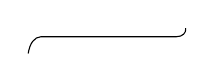
\begin{tikzpicture}[x=.4cm,y=.4cm,baseline=-.2ex]\draw (0,-.35) .. controls (.05,-.02) and (.2,.17) .. (.4,.18)--(4.7,.18) .. controls (4.90,.18) and (5.02,.3) .. (5.00,.45);\end{tikzpicture}}} \uline{exacts et} $k$-\uline{linéaires}, munis d'un isomorphisme $c:G(X\otimes Y)\handwritten{\simeq}G(X)\otimes G(Y)$. \deleted{\unsure{son}} Tout d'abord la donnée de $G^{\deleted{k}}$ exact à droite\inserted{$C\handwritten{\to}\mathrm{Mod}(k')$}\handwritten{\begin{tikzpicture}[x=.4cm,y=.4cm,baseline=-.2ex]\draw (0,-.35) .. controls (.05,-.02) and (.2,.17) .. (.4,.18)--(2.5,.18) .. controls (2.70,.18) and (2.82,.3) .. (2.80,.45);\end{tikzpicture}} revient à la donnée d'un $\rlap{(}L=(L_{\handwritten{\alpha}})$, module\inserted{à droite\handwritten{\begin{tikzpicture}[x=.4cm,y=.4cm,baseline=-.2ex]\draw (0,-.35) .. controls (.05,-.02) and (.2,.17) .. (.4,.18)--(1.4,.18) .. controls (1.60,.18) and (1.72,.3) .. (1.70,.45);\end{tikzpicture}}} sur $U$\handwritten{,} muni d'une structure de $k'$-module \deleted{sur $k$} commutant aux opérations de $U$ (NB $L_{\handwritten{\alpha}}=G(U_{\handwritten{\alpha}\unsure{s|S}})$ ), par
\[
G(\unsure{\rlap{\(X\)}M|\mathbb M})=L\otimes_U\rlap{\(X\)}M.
\]

% source lines 14--23
La $k^{\deleted{\unsure{'}}}$-linéarite signifie que les deux structures sur $k$ de $L$ coïncident, i.e. que $L$ provient d'un\deleted{e} module (pro) sur $U'=(U'_{\handwritten{\alpha}})$ (chaque $L_{\handwritten{\alpha}}$ est un module sur $U'_{\handwritten{\alpha}}$).\inserted{On peut alors écrire $G(X)=L\otimes_{\mathbb U'}X'$, où $X'=X\otimes_kk'$.\handwritten{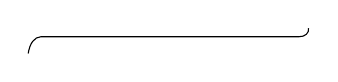
\begin{tikzpicture}[x=.4cm,y=.4cm,baseline=-.2ex]\draw (0,-.35) .. controls (.05,-.02) and (.2,.17) .. (.4,.18)--(8.6,.18) .. controls (8.80,.18) and (8.92,.3) .. (8.90,.45);\end{tikzpicture}}} Le fait que l'on s'envoie dans $\mathrm{Projf}(k')$ \deleted{s'exprime} et que le foncteur envisagé $G$ est exact s'exprime alors par le fait que les $L_{\handwritten{\alpha}}$ sont \deleted{libres}\inserted{proj.} de type fini \uline{sur} $k'$, et que les $L_{\handwritten{\unsure{\alpha|\mu}}}$ sont p\rlap{r}l\rlap{e}ats s\uline{ur les} $U_{\handwritten{\alpha}}$ (nécessité triviale, suffisance un petit argument par réduction au cas $X$ simple, puis $U$ un corps égal à $X$ \ldots). Donc on trouve exactement les \uline{modules} $L=(L_{\handwritten{\alpha}})$ \uline{sur} $U'$ \uline{tels que les} $\handwritten{L_\alpha}$ \uline{soient plats sur} $U_{\handwritten{\alpha}}$ \uline{et proj de tf sur} $k'$.
\margin{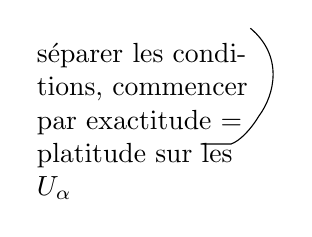
\begin{tikzpicture}[x=.35cm,y=.35cm,baseline=(n.base)]\node[anchor=north west,align=left,text width=3cm] (n) at (0,0) {séparer les conditions, commencer par exactitude = platitude \handwritten{sur les $U_\alpha$}};\draw (8.1,.2) .. controls (9.3,-.8) and (9.0,-2.2) .. (8.4,-3.0) .. controls (8.1,-3.5) and (7.7,-3.9) .. (7.4,-4.0)--(6.3,-4.0);\end{tikzpicture}}
$\mathbb{D}$'$\mathbb{a}\mathbb{u}\mathbb{t}$re part, indépendamment de ces \deleted{C}\inserted{\handwritten{\unsure{c}}\handwritten{\begin{tikzpicture}[x=.4cm,y=.4cm,baseline=-.2ex]\draw (0,.23)--(.14,0)--(.3,.21);\end{tikzpicture}}}onditions de platitude,\inserted{\handwritten{si dans $C$ il y a $1$ et $\vee$ comp.tibles avec\inserted{(\unsure{contravariété|contravariants})}\handwritten{\begin{tikzpicture}[x=.4cm,y=.4cm,baseline=-.2ex]\draw (0,-.35) .. controls (.05,-.02) and (.2,.17) .. (.4,.18)--(3.1,.18) .. controls (3.30,.18) and (3.42,.3) .. (3.40,.45);\end{tikzpicture}} $F$, i.e. $\Delta_U$ unitaire et $U$ avec antipodisme}} la donnée d'un isomorphisme $c$ revient à la donnée d'un isomorphisme de bi-$U'$-modules\inserted{\handwritten{à droite (*)}}
\margin{\deleted{\handwritten{\unsure{en le dualisant} \unsure{faisant intervenir} \illegible{2} d'un \unsure{antipodisme} $\unsure{U'}$}}}
\[
L\overset{\handwritten{\scriptscriptstyle\wedge}}{\otimes}_{\handwritten{k'}}L\handwritten{\xleftarrow{\sim}}L\overset{\handwritten{\scriptscriptstyle\wedge}}{\otimes}_{\handwritten{k'}}U'
\quad(\handwritten{\unsure{\simeq|\xrightarrow{\sim}}}L\otimes_{(U,\handwritten{\Delta})}(U\overset{\handwritten{\scriptscriptstyle\wedge}}{\otimes}_kU)\deleted{\handwritten{\unsure{\simeq}}}\handwritten{\simeq}L\otimes_{(U',\handwritten{\Delta'})}(U'\overset{\handwritten{\scriptscriptstyle\wedge}}{\otimes}_kU')).
\]
\inserted{\handwritten{[grâce à l'antipodisme:) $x\otimes\unsure{U|u}\longrightarrow x\otimes(u\otimes1)$]}\handwritten{\begin{tikzpicture}[x=.4cm,y=.4cm,baseline=-.2ex]\draw (0,-.35) .. controls (.05,-.02) and (.2,.17) .. (.4,.18)--(3.2,.18) .. controls (3.40,.18) and (3.52,.3) .. (3.50,.45);\end{tikzpicture}}}

% source lines 24--26 and lower-margin notes
\deleted{En termes} Utilisant les conditions de platitude, on peut définir $B=\mathrm{Homcont}_{k'}(L,k')$, qui est limite inductive des $B_{\handwritten{\alpha}}$ proj de tf sur $k'$ (à fortiori\inserted{\handwritten{il est}\handwritten{\begin{tikzpicture}[x=.4cm,y=.4cm,baseline=-.2ex]\draw (0,-.35) .. controls (.05,-.02) and (.2,.17) .. (.4,.18)--(1.4,.18) .. controls (1.60,.18) and (1.72,.3) .. (1.70,.45);\end{tikzpicture}}} plat sur $k'$), et une coa\deleted{g}l\`{g}èbre sur $A'$ (limite de coalgèbres
\margin{\begin{tikzpicture}[x=.35cm,y=.35cm,baseline=(n.base)]\node[anchor=north west,align=left,text width=3.4cm] (n) at (0,0) {\handwritten{Commençons \unsure{$U\to$|par} tout exprimer du côté de $U,L$, et ne \handwritten{\begin{tikzpicture}[x=.4cm,y=.4cm,baseline=-.2ex]\draw[line width=.3pt] (.08,.28)--(.07,.02) .. controls (.15,-.11) and (.3,.02) .. (.35,.2)--(.43,-.06);\draw[line width=.55pt] (0,-.14)--(.32,.19);\fill[gray] (.08,.4) circle (.025);\end{tikzpicture}} dualisons qu'à la fin}};\draw (7.2,.8) .. controls (9.2,.7) and (8.8,-1.6) .. (9.7,-2.7) .. controls (10.2,-4.3) and (9.5,-5.8) .. (8.6,-6.8);\draw[line width=.2pt] (10.2,3.5) .. controls (10.1,1.0) and (10.6,-3.0) .. (10.4,-7.2);\end{tikzpicture}}
\handwritten{(*) La loi de bim. dans $L\otimes_{\unsure{U'|k'}}U'$ est donnée par}
\[
\handwritten{\left\{\begin{aligned}
&\text{1ère loi : à droite des }\unsure{\text{mult.}}\text{ de }U'\\
&\text{2ème loi : donnée par celle de mod : droit}\\
&\text{sur }U\otimes U^o\quad[U^o\text{ opère à droite sur }U'\text{ !}]\\
&\text{via }(\mathrm{id}_U\otimes\underline{a}.)(\Delta_U)
\end{aligned}\right.}
\]
